\providecommand{\qcOne}{\mathbf{1}}   %
\providecommand{\qcTwo}{\mathbf{2}}   %
\providecommand{\qcThree}{\mathbf{3}} %
\providecommand{\qcFour}{\mathbf{4}}  %
\providecommand{\qcor}[1]{\ulcorner#1\urcorner}   %
\providecommand{\cellpair}[5]{$\vcenter{\hbox{\begin{tikzpicture}[x=1.15em,y=1.15em]%
\node (s) at (0,0) {$#1$};%
\node (t) at (4.2,0) {$#2$};%
\draw[->] (0.75,0.32) to[bend left=18] (3.45,0.32);%
\node at (2.1,0.88) {$\scriptstyle#3$};%
\draw[->] (0.75,-0.32) to[bend right=18] (3.45,-0.32);%
\node at (2.1,-0.93) {$\scriptstyle#4$};%
\draw[->] (1.95,0.2) to[bend right=32] (1.95,-0.2);%
\node at (2.85,0) {$\scriptstyle#5$};%
\end{tikzpicture}}}$\ignorespaces}

\section{笛卡尔箭头}\label{sec:cartesian-arrows}

在定义\textbf{\trCartesianFibration}（cartesian fibration）这一概念之前，我们先来
描述某些「楼上」的%
\trNaturalTransformation{}所享有的弱\trUniversalProperty。回忆：由第 3 章中的%
\cref{prop:arrow-category-uniqueness}，任何形如下式的\trNaturalTransformation{}
\cellpair{X}{E}{e'}{e}{\psi}
都由一个\trFunctor{} $\qcor{\psi}\colon X\to E^{2}$ 所表示，满足 $p_{0}\qcor{\psi}=e'$
与 $p_{1}\qcor{\psi}=e$，并且诸表示在\trFiberedIsomorphism{}之下唯一。$E$ 中这个%
表示性的 $X$-形箭头 $\qcor{\psi}$ 在\trFunctorSpace{} $\mathrm{Fun}(X,E)$ 中定义了%
一条从 $e'$ 到 $e$ 的 1-箭头（亦称 1-\trSimplex）。

\begin{definition}[$p$-笛卡尔箭头]\label{def:pcartesian-arrow}
设 $p\colon E\twoheadrightarrow B$ 为一条\trIsofibration。$E$ 中的一条 $X$-形箭头%
$\qcor{\psi}\colon X\to E^{2}$ 是\textbf{$p$-\trCartesian}，若由%
\trLeibnizCotensor{}的\trPullback{}所定义的虚线映射是一条\trTrivialFibration：
\begin{center}
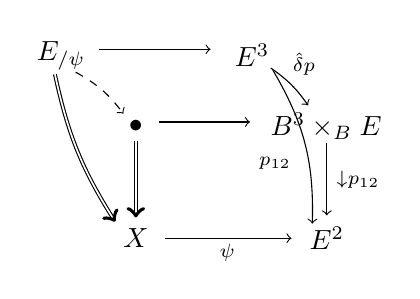
\begin{tikzpicture}[x=1.5em,y=1.5em]
  \node (Ep) at (0,2.7) {$E_{/\psi}$};
  \node (E3) at (4.6,2.7) {$E^{3}$};
  \node (dt) at (1.8,1.0) {$\bullet$};
  \node (BB) at (6.4,1.0) {$B^{3}\times_{B^{\llcorner}}E^{\llcorner}$};
  \node (X)  at (1.8,-1.7) {$X$};
  \node (E2) at (6.4,-1.7) {$E^{2}$};
  \draw[->] (0.9,2.85) -- (3.6,2.85);
  \node at (2.25,3.15) {$\scriptstyle\llcorner$};
  \draw[->,dashed] (0.35,2.3) to[bend left=12] (1.5,1.3);
  \draw[->] (2.35,1.1) -- (4.55,1.1);
  \node at (3.45,1.4) {$\scriptstyle\llcorner$};
  \draw[->] (5.05,2.4) to[bend left=10] (5.95,1.5);
  \node at (5.85,2.5) {$\scriptstyle\hat{\delta}p$};
  \draw[->] (6.4,0.6) -- (6.4,-1.15);
  \node at (7.15,-0.3) {$\scriptstyle\downarrow p_{12}$};
  \draw[->] (5.1,2.35) to[bend left=16] (6.05,-1.35);
  \node at (5.15,0.1) {$\scriptstyle p_{12}$};
  \draw[double,->] (-0.15,2.25) to[bend right=10] (1.3,-1.3);
  \draw[double,->] (1.8,0.65) -- (1.8,-1.2);
  \draw[->] (2.5,-1.7) -- (5.55,-1.7);
  \node at (4.0,-2.05) {$\scriptstyle\qcor{\psi}$};
\end{tikzpicture}
\end{center}
其中 $\delta\colon\llcorner\hookrightarrow\qcThree$是其像为 $\qcThree$ 中%
\trCospan{} $0\to 2\leftarrow 1$ 的那个包含，而 $p_{12}$ 定义为沿包含%
$i_{12}\colon\qcTwo\hookrightarrow\qcThree$的限制，其像即下标所示。
\end{definition}

余定义域为 $E$ 的一条\trNaturalTransformation{}
\cellpair{X}{E}{e'}{e}{\psi}
是 $p$-\trCartesian，若表示它的每一个\trFunctor{} $\qcor{\psi}\colon X\to E^{2}$
都是 $p$-\trCartesian。由练习 3.3.i，这一说法是良定的。我们将在\trNaturalTransformation{}%
$\psi\colon e'\Rightarrow e$ 所呈现的视角与表示箭头 $\qcor{\psi}\colon X\to E^{2}$
所呈现的视角之间自由切换。\footnote{我们也沿用一套精简记号：把警告 4.2.10 中以记号%
$E_{/\qcor{\psi}}$定义的\trInfinityCategory{}径写作 $E_{/\psi}$，并把复合箭头%
$p^{2}\qcor{\psi}$与 $\qcor{\psi}f$分别写作 $\qcor{p^{2}\psi}$与 $\qcor{\psi f}$。}
存在多种彼此等价的方式来陈述 $p$-笛卡尔箭头的定义。

\begin{lemma}\label{lem:dashed-square-hypercube}
对任意\trIsofibration{} $p\colon E\twoheadrightarrow B$，余定义域为%
$e\colon X\to E$的一支箭头 $\qcor{\psi}\colon X\to E^{2}$ 是 $p$-\trCartesian，
当且仅当由超立方体
\begin{rveq}\label{eq:hypercube-weakly-cartesian}
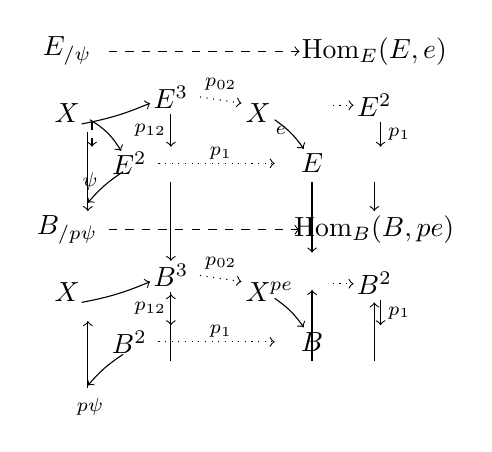
\begin{tikzpicture}[x=1.5em,y=1.5em]
  \node (Ep) at (0,5.2) {$E_{/\psi}$};
  \node (HE) at (7.4,5.2) {$\mathrm{Hom}_{E}(E,e)$};
  \draw[->,dashed] (1.0,5.2) -- (5.6,5.2);
  \node (Xa) at (0,3.7) {$X$};
  \node (E3) at (2.5,4.1) {$E^{3}$};
  \node (Xb) at (4.6,3.7) {$X$};
  \node (E2a) at (7.4,3.9) {$E^{2}$};
  \node (E2b) at (1.5,2.5) {$E^{2}$};
  \node (Eob) at (5.9,2.5) {$E$};
  \draw[->] (0.35,3.45) to[bend right=6] (2.0,3.95);
  \draw[->,dashed] (0.6,3.5) -- (0.6,2.9);
  \draw[->] (0.55,3.55) to[bend left=14] (1.3,2.8);
  \draw[->,dotted] (3.2,4.1) -- node[above]{$\scriptstyle p_{02}$} (4.2,3.95);
  \draw[->,dotted] (6.4,3.9) -- (6.9,3.9);
  \draw[->] (5.0,3.55) to[bend left=10] (5.7,2.85);
  \node at (5.15,3.3) {$\scriptstyle e$};
  \draw[->] (7.55,3.5) -- (7.55,2.9);
  \node at (8.0,3.2) {$\scriptstyle p_{1}$};
  \draw[->] (2.5,3.7) -- (2.5,2.9);
  \node at (2.0,3.3) {$\scriptstyle p_{12}$};
  \draw[->,dotted] (2.2,2.5) -- (5.0,2.5);
  \node at (3.7,2.75) {$\scriptstyle p_{1}$};
  \draw[->] (1.35,2.3) to[bend right=8] (0.5,1.55);
  \node at (0.55,2.05) {$\scriptstyle\qcor{\psi}$};
  \node (Bp) at (0,0.9) {$B_{/p\psi}$};
  \node (HB) at (7.4,0.9) {$\mathrm{Hom}_{B}(B,pe)$};
  \draw[->,dashed] (1.0,0.9) -- (5.6,0.9);
  \node (Xc) at (0,-0.6) {$X$};
  \node (B3) at (2.5,-0.2) {$B^{3}$};
  \node (Xd) at (4.6,-0.6) {$X$};
  \node (B2a) at (7.4,-0.4) {$B^{2}$};
  \node (B2b) at (1.5,-1.8) {$B^{2}$};
  \node (Bb) at (5.9,-1.8) {$B$};
  \draw[->] (0.35,-0.85) to[bend right=6] (2.0,-0.35);
  \draw[->,dotted] (3.2,-0.2) -- node[above]{$\scriptstyle p_{02}$} (4.2,-0.35);
  \draw[->,dotted] (6.4,-0.4) -- (6.9,-0.4);
  \draw[->] (5.0,-0.75) to[bend left=10] (5.7,-1.45);
  \node at (5.15,-0.5) {$\scriptstyle pe$};
  \draw[->] (7.55,-0.8) -- (7.55,-1.4);
  \node at (8.0,-1.1) {$\scriptstyle p_{1}$};
  \draw[->] (2.5,-0.6) -- (2.5,-1.4);
  \node at (2.0,-1.0) {$\scriptstyle p_{12}$};
  \draw[->,dotted] (2.2,-1.8) -- (5.0,-1.8);
  \node at (3.7,-1.55) {$\scriptstyle p_{1}$};
  \draw[->] (1.35,-2.1) to[bend right=8] (0.5,-2.85);
  \node at (0.55,-3.35) {$\scriptstyle\qcor{p\psi}$};
  \draw[->] (0.5,-2.9) -- (0.5,-1.3);
  \draw[->] (2.5,-2.25) -- (2.5,-0.65);
  \draw[->] (5.9,-2.25) -- (5.9,-0.55);
  \draw[->] (7.4,-2.25) -- (7.4,-0.85);
  \draw[->] (0.5,3.25) -- (0.5,1.35);
  \draw[->] (2.5,2.05) -- (2.5,0.15);
  \draw[->] (5.9,2.05) -- (5.9,0.35);
  \draw[->] (7.4,2.05) -- (7.4,1.35);
\end{tikzpicture}
\end{rveq}
所诱导的虚线方块是\trWeaklyCartesianSquare，也就是说，其诱导映射是一条%
\trTrivialFibration：
\[
E_{/\psi}\rightsquigarrow B_{/p\psi}\times_{\mathrm{Hom}_{B}(B,pe)}\mathrm{Hom}_{E}(E,e)
\]
\end{lemma}

\begin{proof}
事实上，虚线方块中诱导出的映射与\cref{def:pcartesian-arrow} 的映射同构。首先注意，%
超立方体 \eqref{eq:hypercube-weakly-cartesian} 中的实线方块都是\trPullback，故由%
超立方体拉回引理\footnote{超立方体拉回引理说的是：形如 $\llcorner\times\llcorner$
的\trDiagram{}的极限，既可先取左因子的诸\trPullback{}再对所得\trCospan{}取%
\trPullback{}而算得，也可先取右因子的诸\trPullback{}再对所得\trCospan{}取%
\trPullback{}而算得。}，虚线方块中的\trPullback{}同样等于图表
\begin{center}
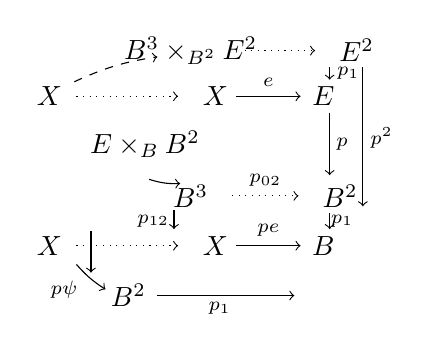
\begin{tikzpicture}[x=1.5em,y=1.5em]
  \node (BE2) at (3.4,2.6) {$B^{3}\times_{B^{2}}E^{2}$};
  \node (E2t) at (7.4,2.6) {$E^{2}$};
  \draw[->,dotted] (4.7,2.6) -- (6.4,2.6);
  \node (Xa) at (0,1.5) {$X$};
  \node (Xb) at (4.0,1.5) {$X$};
  \node (E)   at (6.6,1.5) {$E$};
  \draw[->,dashed] (0.6,1.85) to[bend left=8] (2.6,2.45);
  \draw[->,dotted] (0.65,1.5) -- (3.1,1.5);
  \draw[->] (4.5,1.5) -- node[above]{$\scriptstyle e$} (6.05,1.5);
  \node (EB2) at (2.3,0.35) {$E\times_{B}B^{2}$};
  \draw[->] (6.75,2.2) -- (6.75,1.9);
  \node at (7.2,2.05) {$\scriptstyle p_{1}$};
  \draw[->] (7.55,2.2) -- (7.55,-1.15);
  \node at (8.0,0.5) {$\scriptstyle p^{2}$};
  \draw[->] (6.75,1.1) -- (6.75,-0.4);
  \node at (7.05,0.35) {$\scriptstyle p$};
  \node (B3) at (3.4,-0.9) {$B^{3}$};
  \node (B2t) at (7.0,-0.9) {$B^{2}$};
  \draw[->,dotted] (4.4,-0.9) -- node[above]{$\scriptstyle p_{02}$} (6.0,-0.9);
  \node (Xc) at (0,-2.1) {$X$};
  \node (Xd) at (4.0,-2.1) {$X$};
  \node (B)  at (6.6,-2.1) {$B$};
  \draw[->,dotted] (0.65,-2.1) -- (3.1,-2.1);
  \draw[->] (4.5,-2.1) -- node[above]{$\scriptstyle pe$} (6.05,-2.1);
  \node (B2b) at (1.9,-3.3) {$B^{2}$};
  \draw[->] (1.0,-1.75) -- (1.0,-2.75);
  \draw[->] (0.65,-2.55) to[bend right=8] (1.35,-3.15);
  \node at (0.35,-3.15) {$\scriptstyle\qcor{p\psi}$};
  \draw[->] (2.6,-3.3) -- (5.9,-3.3);
  \node at (4.1,-3.6) {$\scriptstyle p_{1}$};
  \draw[->] (6.75,-1.3) -- (6.75,-1.7);
  \node at (7.05,-1.5) {$\scriptstyle p_{1}$};
  \draw[->] (2.4,-0.5) to[bend right=10] (3.15,-0.6);
  \draw[->] (3.0,-1.25) -- (3.0,-1.7);
  \node at (2.5,-1.5) {$\scriptstyle p_{12}$};
\end{tikzpicture}
\end{center}
的极限，其中此时点线方块是\trPullback。于是，我们的映射同构于某立方体的顶部虚映射%
——该立方体的前面与后面恰是定义其定义域与余定义域的诸\trPullback：
\begin{center}
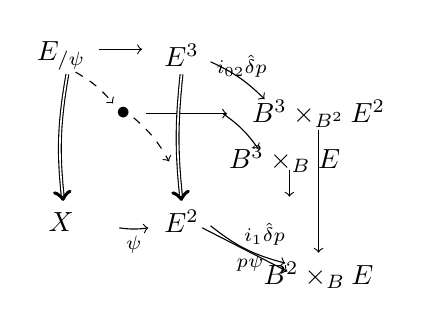
\begin{tikzpicture}[x=1.5em,y=1.5em]
  \node (Ep) at (0,2.4) {$E_{/\psi}$};
  \node (E3) at (2.9,2.4) {$E^{3}$};
  \node (dt) at (1.5,1.0) {$\bullet$};
  \node (BB) at (6.2,1.0) {$B^{3}\times_{B^{2}}E^{2}$};
  \node (mB) at (5.4,-0.1) {$B^{3}\times_{B^{\llcorner}}E^{\llcorner}$};
  \node (X)  at (0,-1.6) {$X$};
  \node (E2) at (2.9,-1.6) {$E^{2}$};
  \node (BX) at (6.2,-2.9) {$B^{2}\times_{B}E$};
  \draw[->] (0.9,2.55) -- (1.95,2.55);
  \node at (1.4,2.85) {$\scriptstyle\llcorner$};
  \draw[->] (3.6,2.25) to[bend left=10] (4.9,1.35);
  \node at (4.35,2.15) {$\scriptstyle i_{02}\hat{\delta}p$};
  \draw[->,dashed] (0.35,2.0) to[bend left=10] (1.25,1.25);
  \draw[->,dashed] (1.75,0.9) to[bend left=10] (2.6,-0.15);
  \draw[->] (2.05,1.0) -- (4.0,1.0);
  \node at (3.0,1.3) {$\scriptstyle\llcorner$};
  \draw[->] (3.9,1.0) to[bend left=10] (4.75,0.15);
  \node at (4.6,0.72) {$\scriptstyle\llcorner$};
  \draw[->] (5.5,-0.35) -- (5.5,-1.0);
  \node at (6.05,-0.7) {$\scriptstyle\llcorner$};
  \draw[->] (6.2,0.6) -- (6.2,-2.35);
  \draw[->] (1.4,-1.75) to[bend right=8] (2.1,-1.75);
  \node at (1.75,-2.15) {$\scriptstyle\qcor{\psi}$};
  \draw[->] (3.6,-1.7) to[bend right=12] (5.4,-2.6);
  \node at (4.9,-1.9) {$\scriptstyle i_{1}\hat{\delta}p$};
  \draw[->] (3.4,-1.75) -- (5.45,-2.8);
  \node at (4.55,-2.6) {$\scriptstyle\qcor{p\psi}$};
  \draw[double,->] (0.15,1.95) to[bend right=8] (0.05,-1.1);
  \draw[double,->] (2.9,1.95) to[bend right=6] (2.9,-1.1);
\end{tikzpicture}
\end{center}
到右面中\trPullback{}的诱导映射是 $\hat{\delta}p\colon E^{3}\to B^{3}\times_{B^{\llcorner}}E^{\llcorner}$，
这可以通过再构造一个超立方体来验证。由\trPullback{}的复合与消去，此映射经拉回即得%
左面中的虚映射；但由于底边是恒同，它与顶部虚映射重合。注意，%
\cref{def:pcartesian-arrow}中展示的图表作为后棱柱嵌入在这个立方体中。
\end{proof}

接下来的几条引理将为相对于固定\trIsofibration{} $p\colon E\twoheadrightarrow B$
而定义的 $p$-笛卡尔变换类发展出若干稳定性性质。

\begin{lemma}[限制下的稳定性]\label{lem:stability-under-restriction}
若 $\qcor{\psi}\colon X\to E^{2}$ 是 $p$-\trCartesian，则它沿任何\trFunctor{}%
$f\colon Y\to X$的限制亦然。
\end{lemma}

\begin{proof}
由\cref{def:pcartesian-arrow}，若 $\psi$ 是 $p$-\trCartesian，我们便有一条%
\trTrivialFibration
\begin{center}
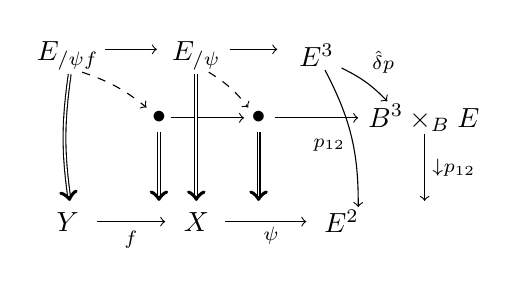
\begin{tikzpicture}[x=1.5em,y=1.5em]
  \node (Epf) at (0,2.5) {$E_{/\psi f}$};
  \node (Ep)  at (3.1,2.5) {$E_{/\psi}$};
  \node (E3)  at (6.0,2.5) {$E^{3}$};
  \node (d1)  at (2.2,1.0) {$\bullet$};
  \node (d2)  at (4.6,1.0) {$\bullet$};
  \node (BB)  at (8.6,1.0) {$B^{3}\times_{B^{\llcorner}}E^{\llcorner}$};
  \node (Y)   at (0,-1.5) {$Y$};
  \node (X)   at (3.1,-1.5) {$X$};
  \node (E2)  at (6.6,-1.5) {$E^{2}$};
  \draw[->] (0.9,2.65) -- (2.15,2.65);
  \node at (1.5,2.95) {$\scriptstyle\llcorner$};
  \draw[->] (3.9,2.65) -- (5.05,2.65);
  \node at (4.5,2.95) {$\scriptstyle\llcorner$};
  \draw[->] (6.6,2.2) to[bend left=10] (7.7,1.4);
  \node at (7.6,2.35) {$\scriptstyle\hat{\delta}p$};
  \draw[->,dashed] (0.35,2.1) to[bend left=10] (1.9,1.25);
  \draw[->,dashed] (3.4,2.1) to[bend left=10] (4.35,1.25);
  \draw[->] (2.5,1.0) -- (4.25,1.0);
  \node at (3.4,1.3) {$\scriptstyle\llcorner$};
  \draw[->] (5.0,1.0) -- (7.0,1.0);
  \node at (6.0,1.3) {$\scriptstyle\llcorner$};
  \draw[->] (8.6,0.6) -- (8.6,-1.0);
  \node at (9.3,-0.2) {$\scriptstyle\downarrow p_{12}$};
  \draw[->] (6.2,2.15) to[bend left=14] (7.0,-1.15);
  \node at (6.3,0.35) {$\scriptstyle p_{12}$};
  \draw[double,->] (0.05,2.05) to[bend right=8] (0.05,-1.0);
  \draw[double,->] (3.1,2.05) -- (3.1,-1.0);
  \draw[double,->] (2.2,0.65) -- (2.2,-1.0);
  \draw[double,->] (4.6,0.65) -- (4.6,-1.0);
  \draw[->] (0.7,-1.5) -- node[below]{$\scriptstyle f$} (2.35,-1.5);
  \draw[->] (3.8,-1.5) -- (5.75,-1.5);
  \node at (4.9,-1.85) {$\scriptstyle\qcor{\psi}$};
\end{tikzpicture}
\end{center}
它经拉回定义出一条\trTrivialFibration，后者表明 $\qcor{\psi f}$ 是一支%
$p$-\trCartesian{}箭头。
\end{proof}

我们现在来证明：$p$-笛卡尔变换类在\trHomotopyTwoCategory{}中对竖复合与左消去封闭。

\begin{lemma}\label{lem:left-cancellation}
设 $p\colon E\twoheadrightarrow B$ 为\trIsofibration，并考虑满足%
$\psi''=\psi\cdot\psi'$的一些\trNaturalTransformation，其中 $\psi$ 是%
$p$-\trCartesian。则 $\psi'$ 是 $p$-\trCartesian，当且仅当 $\psi''$ 是%
$p$-\trCartesian。
\end{lemma}

\begin{proof}
由第 1 章中的引理 1.1.12，对任意代表满足 $\psi''=\psi\cdot\psi'$的%
\trNaturalTransformation{}的三支箭头 $\qcor{\psi''}$、$\qcor{\psi'}$、%
$\qcor{\psi}\colon X\to E^{3}$，存在 $\mathrm{Fun}(X,E)$ 中的一个%
2-\trSimplex，它由一个\trFunctor{} $\qcor{\tau}\colon X\to E^{3}$ 所表示，
其边界恰由这些指定的表示函子给出：
\begin{center}
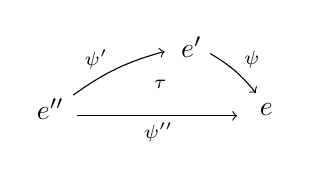
\begin{tikzpicture}[x=1.5em,y=1.5em]
  \node (epp) at (0,0) {$e''$};
  \node (ep)  at (3.4,1.5) {$e'$};
  \node (e)   at (5.2,0) {$e$};
  \draw[->] (0.55,0.35) to[bend left=10] (2.75,1.4);
  \node at (1.1,1.2) {$\scriptstyle\psi'$};
  \draw[->] (3.85,1.35) to[bend left=10] (4.95,0.4);
  \node at (4.85,1.2) {$\scriptstyle\psi$};
  \draw[->] (0.65,-0.15) -- (4.5,-0.15);
  \node at (2.6,-0.55) {$\scriptstyle\psi''$};
  \node at (2.65,0.6) {$\scriptstyle\tau$};
\end{tikzpicture}
\end{center}
通过把左下的范畴图表\trCotensor{}入 $E$、限制到始顶点 $0\in\qcOne$的补、再沿%
$\qcor{\tau}\colon X\to E^{3}$及其面拉回，我们得到右下的∞-范畴图表，其中底部%
方块是\trWeaklyCartesianSquare（关于外跨度之构造以及 $p_{01}$ 皆为%
\trTrivialFibration{}的证明，详见第 4 章中的引理 4.3.9）。
\begin{center}
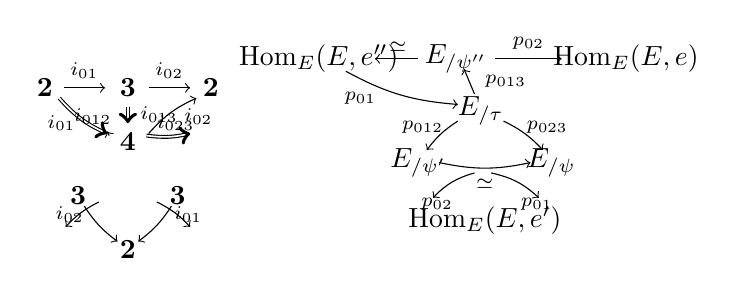
\begin{tikzpicture}[x=1.5em,y=1.5em]
  \node (t2a) at (0,2.2) {$\qcTwo$};
  \node (t3a) at (2.0,2.2) {$\qcThree$};
  \node (t2b) at (4.0,2.2) {$\qcTwo$};
  \draw[->] (0.45,2.2) -- node[above]{$\scriptstyle i_{01}$} (1.45,2.2);
  \draw[->] (2.5,2.2) -- node[above]{$\scriptstyle i_{02}$} (3.5,2.2);
  \node (t4) at (2.0,0.9) {$\qcFour$};
  \draw[double,->] (2.0,1.75) -- (2.0,1.35);
  \node at (2.75,1.55) {$\scriptstyle i_{013}$};
  \draw[double,->] (0.35,1.95) to[bend right=12] (1.5,1.1);
  \node at (0.4,1.35) {$\scriptstyle i_{01}$};
  \draw[->] (1.55,1.05) -- (1.5,1.15);
  \node at (1.15,1.5) {$\scriptstyle i_{012}$};
  \draw[->] (2.5,1.1) to[bend left=12] (3.65,1.95);
  \node at (3.7,1.5) {$\scriptstyle i_{02}$};
  \draw[double,->] (2.45,1.05) to[bend right=10] (3.5,1.1);
  \node at (3.15,1.35) {$\scriptstyle i_{023}$};
  \node (t3b) at (0.8,-0.4) {$\qcThree$};
  \node (t3c) at (3.2,-0.4) {$\qcThree$};
  \draw[->] (1.3,-0.55) to[bend right=10] (0.5,-1.15);
  \node at (0.6,-0.85) {$\scriptstyle i_{02}$};
  \draw[->] (2.7,-0.55) to[bend left=10] (3.5,-1.15);
  \node at (3.45,-0.85) {$\scriptstyle i_{01}$};
  \node (t2c) at (2.0,-1.7) {$\qcTwo$};
  \draw[->] (0.95,-0.65) to[bend right=10] (1.75,-1.5);
  \draw[->] (3.05,-0.65) to[bend left=10] (2.25,-1.5);
  \node at (5.5,0.4) {$\rightsquigarrow$};
  \begin{scope}[shift={(6.6,0.9)}]
  \node (HE2) at (0,2.0) {$\mathrm{Hom}_{E}(E,e'')$};
  \node (E2p) at (3.3,2.0) {$E_{/\psi''}$};
  \node (HE3) at (7.4,2.0) {$\mathrm{Hom}_{E}(E,e)$};
  \draw[->] (2.4,2.0) -- (1.35,2.0);
  \node at (1.9,2.3) {$\scriptstyle\simeq$};
  \draw[->] (4.25,2.0) -- node[above]{$\scriptstyle p_{02}$} (5.85,2.0);
  \node (Et) at (3.9,0.75) {$E_{/\tau}$};
  \draw[->] (3.75,1.15) -- (3.5,1.75);
  \node at (4.5,1.45) {$\scriptstyle p_{013}$};
  \node (Epp) at (2.4,-0.5) {$E_{/\psi'}$};
  \node (Eps) at (5.6,-0.5) {$E_{/\psi}$};
  \draw[->] (3.35,0.5) to[bend right=10] (2.6,-0.2);
  \node at (2.5,0.35) {$\scriptstyle p_{012}$};
  \draw[->] (4.45,0.5) to[bend left=10] (5.4,-0.2);
  \node at (5.5,0.35) {$\scriptstyle p_{023}$};
  \draw[->] (0.65,1.7) to[bend right=12] (3.35,0.9);
  \node at (1.0,1.05) {$\scriptstyle p_{01}$};
  \draw[->] (3.75,-0.75) to[bend right=15] (2.75,-1.35);
  \node at (2.85,-1.5) {$\scriptstyle p_{02}$};
  \draw[->] (4.15,-0.75) to[bend left=15] (5.3,-1.35);
  \node at (5.25,-1.5) {$\scriptstyle p_{01}$};
  \draw[->] (2.9,-0.5) to[bend right=12] (5.1,-0.5);
  \node at (4.0,-1.0) {$\scriptstyle\simeq$};
  \node (HE1) at (4.0,-1.9) {$\mathrm{Hom}_{E}(E,e')$};
  \end{scope}
\end{tikzpicture}
\end{center}
\trIsofibration{} $p\colon E\twoheadrightarrow B$定义了从这个图表到为%
$\qcor{p\tau}\colon X\to B^{3}$构造的类似图表的一个\trNaturalTransformation。%
\footnote{构造此图的更佳途径，是把这一构造实现在由第 6 章中的命题 6.1.1 定义的%
\trIsofibration\trInfinityCosmos{}中；这还额外告诉我们，每个自然性方块中到%
\trPullback{}的映射都是\trIsofibration。}
\cref{lem:dashed-square-hypercube}的\trTrivialFibration{}
$E_{/\psi}\twoheadrightarrow B_{/p\psi}\times_{\mathrm{Hom}_{B}(B,pe)}\mathrm{Hom}_{E}(E,e)$
经拉回定义出下图中展示的虚\trTrivialFibration，它与来自 $E_{/\tau}$ 的诱导映射交换：
\begin{center}
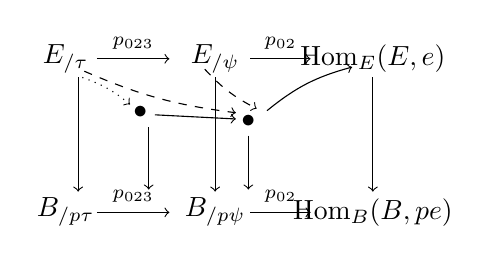
\begin{tikzpicture}[x=1.5em,y=1.5em]
  \node (Et) at (0,2.4) {$E_{/\tau}$};
  \node (Eps) at (3.6,2.4) {$E_{/\psi}$};
  \node (HE)  at (7.4,2.4) {$\mathrm{Hom}_{E}(E,e)$};
  \draw[->] (0.75,2.4) -- node[above]{$\scriptstyle p_{023}$} (2.5,2.4);
  \draw[->] (4.45,2.4) -- node[above]{$\scriptstyle p_{02}$} (5.9,2.4);
  \node (d1) at (1.8,1.1) {$\bullet$};
  \node (d2) at (4.4,0.9) {$\bullet$};
  \draw[->,dotted] (0.4,1.95) to[bend left=10] (1.55,1.3);
  \draw[->,dashed] (0.45,2.1) to[bend right=8] (4.1,1.1);
  \draw[->,dashed] (3.35,2.15) to[bend right=10] (4.6,1.2);
  \draw[->] (2.15,1.05) -- (4.1,0.95);
  \node at (3.1,1.3) {$\scriptstyle\llcorner$};
  \draw[->] (4.85,1.15) to[bend left=12] (6.9,2.2);
  \node at (5.7,1.4) {$\scriptstyle\llcorner$};
  \node (Bpt) at (0,-1.3) {$B_{/p\tau}$};
  \node (Bps) at (3.6,-1.3) {$B_{/p\psi}$};
  \node (HB)  at (7.4,-1.3) {$\mathrm{Hom}_{B}(B,pe)$};
  \draw[->] (0.75,-1.3) -- node[above]{$\scriptstyle p_{023}$} (2.5,-1.3);
  \draw[->] (4.45,-1.3) -- node[above]{$\scriptstyle p_{02}$} (5.9,-1.3);
  \draw[->] (0.3,1.95) -- (0.3,-0.8);
  \draw[->] (3.6,1.95) -- (3.6,-0.8);
  \draw[->] (7.4,1.95) -- (7.4,-0.8);
  \draw[->] (2.0,0.75) -- (2.0,-0.75);
  \draw[->] (4.4,0.55) -- (4.4,-0.75);
\end{tikzpicture}
\end{center}
由等价的\trTwoOfThreeProperty，若两条点线映射中任一条是\trTrivialFibration，
则另一条亦是。
\end{proof}

这些图表诱导出一个交换方块，展示于立方体内部——从上方的点线映射指向检测%
$\psi'$是否 $p$-笛卡尔的那条映射：
\begin{center}
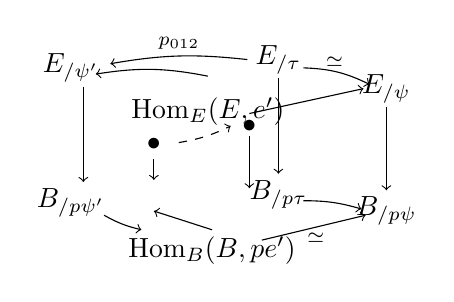
\begin{tikzpicture}[x=1.5em,y=1.5em]
  \node (Epp) at (0,2.4) {$E_{/\psi'}$};
  \node (Et)  at (5.0,2.6) {$E_{/\tau}$};
  \node (Eps) at (7.6,1.9) {$E_{/\psi}$};
  \draw[->] (4.25,2.6) to[bend right=8] (0.95,2.5);
  \node at (2.6,3.0) {$\scriptstyle p_{012}$};
  \draw[->] (5.6,2.4) to[bend left=12] (7.2,2.0);
  \node at (6.35,2.55) {$\scriptstyle\simeq$};
  \node (HE1) at (3.3,1.35) {$\mathrm{Hom}_{E}(E,e')$};
  \draw[->] (3.3,2.2) to[bend right=10] (0.6,2.25);
  \draw[->] (4.3,1.3) -- (7.05,1.9);
  \node at (4.3,1.0) {$\bullet$};
  \node at (2.0,0.55) {$\bullet$};
  \draw[->,dashed] (2.6,0.6) to[bend right=8] (3.85,1.0);
  \node at (3.2,1.05) {$\scriptstyle\rightsquigarrow$};
  \draw[->] (0.3,1.95) -- (0.3,-0.35);
  \draw[->] (5.0,2.15) -- (5.0,-0.15);
  \draw[->] (7.6,1.45) -- (7.6,-0.55);
  \node (Bpp) at (0,-0.85) {$B_{/p\psi'}$};
  \node (Bpt) at (5.0,-0.65) {$B_{/p\tau}$};
  \node (Bps) at (7.6,-1.05) {$B_{/p\psi}$};
  \draw[->] (0.8,-1.15) to[bend right=8] (1.7,-1.5);
  \draw[->] (5.6,-0.8) to[bend left=8] (7.0,-1.0);
  \node (HB1) at (3.4,-2.0) {$\mathrm{Hom}_{B}(B,pe')$};
  \draw[->] (3.4,-1.5) -- (2.0,-1.05);
  \draw[->] (4.6,-1.75) -- (7.1,-1.15);
  \node at (5.9,-1.7) {$\scriptstyle\simeq$};
  \draw[->] (2.0,0.2) -- (2.0,-0.3);
  \node at (1.55,-0.05) {$\scriptstyle\llcorner$};
  \draw[->] (4.3,0.75) -- (4.3,-0.5);
  \node at (3.85,0.1) {$\scriptstyle\llcorner$};
\end{tikzpicture}
\end{center}
由\trTwoOfThreeProperty，这两条映射中若有一条是\trTrivialFibration，另一条亦是。
用$p_{013}\colon E_{/\tau}\twoheadrightarrow E_{/\psi''}$定义的类似方块表明：下方点线%
映射是\trTrivialFibration，当且仅当%
$E_{/\psi''}\twoheadrightarrow B_{/p\psi''}\times_{\mathrm{Hom}_{B}(B,pe)}\mathrm{Hom}_{E}(E,e)$
是。于是，当 $\psi$ 是 $p$-\trCartesian{}时，这些条件彼此等价。

$p$-笛卡尔箭头的同构稳定性由下面这组观察来表达：

\begin{lemma}\label{lem:isomorphism-stability}
设 $p\colon E\twoheadrightarrow B$为\trIsofibration。
\begin{enumerate}[label=(\roman*)]
\item 余定义域为 $E$ 的自然同构定义 $p$-笛卡尔箭头。
\item 自然同构的任一 $p$-笛卡尔提升都是自然同构。
\item $p$-笛卡尔箭头类对与自然同构的\trPreComposition{}与\trPostComposition{}封闭。
\end{enumerate}
\end{lemma}

\begin{proof}
由第 4 章中的引理 4.3.9，$\psi\colon e'\Rightarrow e$是一个\trIsomorphism，
当且仅当定义\cref{lem:dashed-square-hypercube}中\trWeaklyCartesianSquare{}顶部%
水平箭头的映射 $p_{02}\colon E_{/\psi}\to\mathrm{Hom}_{E}(E,e)$是一条%
\trTrivialFibration。
于是若 $\psi$ 可逆，则\cref{lem:dashed-square-hypercube}的两条水平箭头都是%
\trTrivialFibration，该方块自动成为\trWeaklyCartesianSquare，这证明了 (i)。
对于 (ii)，若 $p\psi$ 可逆，则此方块中的底部水平箭头是\trTrivialFibration，
于是当 $\psi$ 是\trWeaklyCartesian{}时，%
$p_{02}\colon E_{/\psi}\to\mathrm{Hom}_{E}(E,e)$是诸\trTrivialFibration{}的%
一个复合，这证明 $\psi$ 可逆。最后的性质 (iii) 由 (i) 与%
\cref{lem:left-cancellation}得到。
\end{proof}

我们从 $p$-笛卡尔箭头的两种更为精细的刻画中获得相当可观的回报。

\begin{theorem}\label{thm:pcartesian-characterizations}
设 $p\colon E\twoheadrightarrow B$为\trIsofibration，$\qcor{\psi}\colon X\to E^{2}$
为表示\trNaturalTransformation{}
\cellpair{X}{E}{e'}{e}{\psi}
的一支箭头。下列诸条等价：
\begin{enumerate}[label=(\roman*)]
\item $\psi$ 是 $p$-\trCartesian。
\item 交换三角形定义出一个绝对右提升图表：
\begin{center}
\begin{tikzpicture}[x=1.5em,y=1.5em]
  \node (E2) at (3.2,1.5) {$E^{2}$};
  \node (X)  at (0,0) {$X$};
  \node (HB) at (3.2,0) {$\mathrm{Hom}_{B}(B,p)$};
  \draw[->] (0.55,0.4) -- node[above,pos=0.6]{$\scriptstyle\qcor{\psi}$} (2.5,1.3);
  \draw[->] (3.2,1.05) -- (3.2,0.45);
  \node at (3.95,0.75) {$\scriptstyle i_{1}\hat{\delta}p$};
  \draw[double,->] (0.7,-0.05) -- (2.4,-0.05);
  \node at (1.5,-0.4) {$\scriptstyle\qcor{p\psi}$};
  \node at (1.5,0.35) {$\scriptstyle\parallel$};
  \node at (5.4,0.7) {其中};
  \begin{scope}[shift={(6.4,0)}]
  \node (E2) at (0.6,2.1) {$E^{2}$};
  \node (B2) at (5.6,1.7) {$B^{2}$};
  \draw[->] (1.35,2.2) to[bend left=12] (4.95,1.85);
  \node at (3.2,2.4) {$\scriptstyle p^{2}$};
  \node (HB) at (2.4,0.8) {$\mathrm{Hom}_{B}(B,p)$};
  \draw[->,dashed] (0.35,1.8) to[bend right=10] (1.7,1.05);
  \node at (0.6,1.15) {$\scriptstyle i_{1}\hat{\delta}p$};
  \draw[->] (3.35,0.85) -- (4.9,1.5);
  \node at (4.15,0.85) {$\scriptstyle\qcor{\phi}$};
  \node at (4.0,1.35) {$\scriptstyle\llcorner$};
  \draw[->] (2.4,0.35) -- (2.4,-0.75);
  \node at (2.0,-0.2) {$\scriptstyle p_{1}$};
  \node (E)  at (2.4,-1.1) {$E$};
  \node (B)  at (5.6,-1.1) {$B$};
  \draw[->] (3.1,-1.1) -- node[below]{$\scriptstyle p$} (4.9,-1.1);
  \draw[->] (5.6,1.25) -- (5.6,-0.65);
  \node at (6.05,0.3) {$\scriptstyle p_{1}$};
  \draw[->] (0.6,1.65) to[bend right=14] (2.15,-0.85);
  \node at (0.55,0.3) {$\scriptstyle p_{1}$};
  \end{scope}
\end{tikzpicture}
\end{center}
\item 存在一个绝对右提升图表，满足 $p_{1}\epsilon=\psi$与 $p_{0}\epsilon=\mathrm{id}_{pe}$：
\begin{center}
\begin{tikzpicture}[x=1.5em,y=1.5em]
  \node (E)  at (3.0,1.5) {$E$};
  \node (X)  at (0,0) {$X$};
  \node (HB) at (3.4,0) {$\mathrm{Hom}_{B}(B,p)$};
  \draw[->] (0.55,0.4) -- node[above,pos=0.55]{$\scriptstyle e'$} (2.45,1.35);
  \node at (1.75,0.62) {$\scriptstyle\psi\epsilon$};
  \draw[->] (3.0,1.05) -- (3.15,0.45);
  \node at (3.8,0.75) {$\scriptstyle\Delta_{p}$};
  \draw[double,->] (0.7,-0.05) -- (2.55,-0.05);
  \node at (1.55,-0.4) {$\scriptstyle\qcor{p\psi}$};
  \node at (5.4,0.7) {其中};
  \begin{scope}[shift={(6.4,0)}]
  \node (E)  at (0.4,2.1) {$E$};
  \node (E2) at (3.4,2.1) {$E^{2}$};
  \draw[->] (1.05,2.25) to[bend left=8] (2.75,2.25);
  \node at (1.9,2.6) {$\scriptstyle\Delta$};
  \draw[->] (4.1,2.2) to[bend left=12] (5.75,1.6);
  \node at (5.1,2.35) {$\scriptstyle p^{2}$};
  \node (B2) at (6.2,1.3) {$B^{2}$};
  \node (HB) at (3.2,0.9) {$\mathrm{Hom}_{B}(B,p)$};
  \draw[->,dashed] (0.5,1.8) to[bend right=10] (2.4,1.1);
  \node at (1.0,1.1) {$\scriptstyle\Delta_{p}$};
  \draw[->] (4.1,0.9) -- (5.75,1.2);
  \node at (4.9,0.65) {$\scriptstyle\qcor{\phi}$};
  \node at (4.7,1.2) {$\scriptstyle\llcorner$};
  \draw[->] (3.2,0.45) -- (3.2,-0.75);
  \node at (2.8,-0.15) {$\scriptstyle p_{1}$};
  \node (E)  at (3.2,-1.1) {$E$};
  \node (B)  at (6.2,-1.1) {$B$};
  \draw[->] (3.9,-1.1) -- node[below]{$\scriptstyle p$} (5.5,-1.1);
  \draw[->] (6.2,0.85) -- (6.2,-0.65);
  \node at (6.65,0.1) {$\scriptstyle p_{1}$};
  \draw[double,->] (0.5,1.65) to[bend right=16] (2.9,-0.85);
  \end{scope}
\end{tikzpicture}
\end{center}
\end{enumerate}
\end{theorem}

从高处着眼，$p$-笛卡尔箭头的这三种刻画之间的等价很容易解释。由%
\cref{def:pcartesian-arrow}与第 3 章中的定理 3.5.3，三条陈述中的每一条%
都断言∞-范畴之间的某个映射是\trEquivalence，而这三个映射结果证明彼此等价。
但这一等价的几何相当微妙，正如证明所揭示的那样。

\begin{proof}
我们证明 (i)$\Rightarrow$(ii)$\Rightarrow$(iii)$\Rightarrow$(i)。

\textbf{(i)$\Rightarrow$(ii)：}我们用\cref{def:pcartesian-arrow}的条件%
证明 $\qcor{\psi}\colon X\to E^{2}$定义出 $\qcor{p\psi}$沿 $i_{1}\hat{\delta}p$
的一个绝对右提升。由定理 3.5.3，我们的任务是证明：由恒同 2-胞腔诱导的%
\trFunctor{}定义出\trCommaInfinityCategory{}之间的一个\trEquivalence。在此%
情形，欲求的映射展示于左下，它是 $p$ 沿包含 $\iota\colon\sqcap\hookrightarrow\square$
的\trLeibnizCotensor{}的\trPullback：
\begin{rveq}\label{eq:pulled-back-leibniz-square}
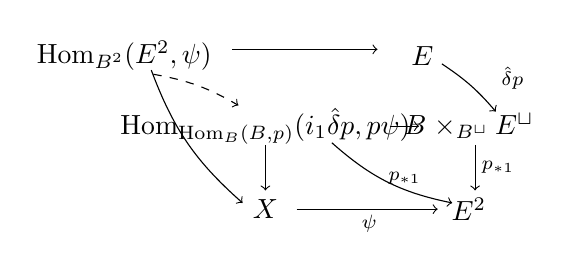
\begin{tikzpicture}[x=1.5em,y=1.5em]
  \node (HB2) at (0,2.4) {$\mathrm{Hom}_{B^{2}}(E^{2},\qcor{\psi})$};
  \node (Esq) at (7.2,2.4) {$E^{\square}$};
  \draw[->] (2.6,2.55) -- (6.1,2.55);
  \node at (4.3,2.85) {$\scriptstyle\llcorner$};
  \draw[->] (7.65,2.2) to[bend left=8] (8.95,1.05);
  \node at (9.35,1.85) {$\scriptstyle\hat{\delta}p$};
  \draw[->,dashed] (0.7,1.95) to[bend left=10] (2.75,1.2);
  \node (HBH) at (3.4,0.7) {$\mathrm{Hom}_{\mathrm{Hom}_{B}(B,p)}(i_{1}\hat{\delta}p,\qcor{p\psi})$};
  \draw[->] (3.4,0.25) -- (3.4,-0.85);
  \node (BB) at (8.3,0.7) {$B^{\square}\times_{B^{\sqcup}}E^{\sqcup}$};
  \draw[->] (6.4,0.7) -- (7.1,0.7);
  \node at (6.85,1.0) {$\scriptstyle\llcorner$};
  \draw[->] (8.45,0.25) -- (8.45,-0.85);
  \node at (9.0,-0.3) {$\scriptstyle p_{*1}$};
  \node (X) at (3.4,-1.3) {$X$};
  \node (E2) at (8.3,-1.3) {$E^{2}$};
  \draw[->] (4.15,-1.3) -- (7.55,-1.3);
  \node at (5.9,-1.65) {$\scriptstyle\qcor{\psi}$};
  \draw[->] (5.0,0.3) to[bend right=15] (7.9,-1.15);
  \node at (6.75,-0.55) {$\scriptstyle p_{*1}$};
  \draw[->] (0.65,2.05) to[bend right=14] (2.85,-1.15);
\end{tikzpicture}
\end{rveq}
由于包含 $\iota$ 可按下左图分解，由附录 C 中的命题 C.2.9(vi)，\trLeibnizCotensor{}%
可按下右图分解：
\begin{center}
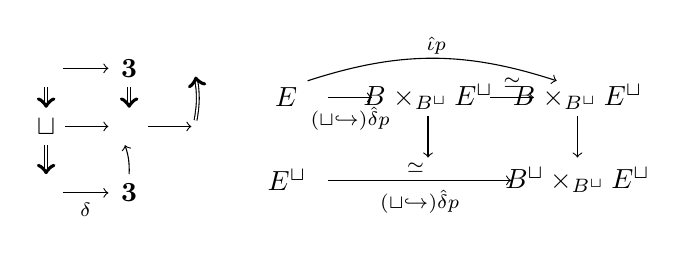
\begin{tikzpicture}[x=1.5em,y=1.5em]
  \node (lc) at (0,1.6) {$\llcorner$};
  \node (t3) at (2.0,1.6) {$\qcThree$};
  \draw[->] (0.4,1.6) -- (1.5,1.6);
  \node (su) at (0,0.2) {$\sqcup$};
  \draw[double,->] (0,1.15) -- (0,0.65);
  \node (bm) at (2.0,0.2) {$\boxminus$};
  \draw[->] (0.45,0.2) -- (1.5,0.2);
  \node at (1.0,0.5) {$\scriptstyle\llcorner$};
  \node (sq) at (4.0,0.2) {$\square$};
  \draw[->] (2.45,0.2) -- (3.5,0.2);
  \node at (3.0,0.5) {$\scriptstyle\llcorner$};
  \draw[double,->] (2.0,1.15) -- (2.0,0.65);
  \draw[double,->] (3.6,0.35) to[bend right=10] (3.6,1.4);
  \node (lc2) at (0,-1.4) {$\llcorner$};
  \draw[double,->] (0,-0.25) -- (0,-0.95);
  \draw[->] (0.4,-1.4) -- node[below]{$\scriptstyle\delta$} (1.5,-1.4);
  \node (t3b) at (2.0,-1.4) {$\qcThree$};
  \draw[->] (2.0,-0.95) to[bend right=10] (1.9,-0.25);
  \node at (4.9,0.1) {$\rightsquigarrow$};
  \begin{scope}[shift={(5.8,0)}]
  \node (Esq) at (0,0.9) {$E^{\square}$};
  \node (Bs1) at (3.4,0.9) {$B^{\square}\times_{B^{\sqcup}}E^{\sqcup}$};
  \node (Bs2) at (7.0,0.9) {$B^{\square}\times_{B^{\sqcup}}E^{\sqcup}$};
  \draw[->] (1.0,0.9) -- node[below]{$\scriptstyle(\sqcup\hookrightarrow\square)\hat{\delta}p$} (2.05,0.9);
  \draw[->] (4.9,0.9) -- node[above]{$\scriptstyle\simeq$} (5.95,0.9);
  \draw[->] (0.5,1.3) to[bend left=18] (6.5,1.3);
  \node at (3.6,2.15) {$\scriptstyle\hat{\iota}p$};
  \draw[->] (3.4,0.45) -- (3.4,-0.55);
  \draw[->] (7.0,0.45) -- (7.0,-0.55);
  \node (Eu) at (0,-1.1) {$E^{\sqcup}$};
  \node (Bu) at (7.0,-1.1) {$B^{\sqcup}\times_{B^{\sqcup}}E^{\sqcup}$};
  \draw[->] (1.0,-1.1) -- node[below]{$\scriptstyle(\sqcup\hookrightarrow\square)\hat{\delta}p$} (5.4,-1.1);
  \node at (3.1,-0.8) {$\scriptstyle\simeq$};
  \end{scope}
\end{tikzpicture}
\end{center}
又由于 $\sqcup\hookrightarrow\square$是某内号角包含的\trPushout，这两支映射中的%
第二支是\trTrivialFibration。由于 $\boxminus\hookrightarrow\square$是 $\delta$
的一个\trPushout，$(\boxminus\hookrightarrow\square)\hat{\delta}p$是%
$\hat{\delta}p$ 的一个\trPullback。由假设 (i)，后一映射沿%
$\qcor{\psi}\colon X\to E^{2}$拉回到一条\trTrivialFibration。于是前一映射亦然，
从而 \eqref{eq:pulled-back-leibniz-square} 中的虚映射是\trTrivialFibration，
这证明了 (ii) 所宣称的绝对提升图。

\textbf{(ii)$\Rightarrow$(iii)：}常值图表函子 $\Delta\colon E\to E^{2}$定义为%
沿函子 $!\colon\qcTwo\to\qcOne$的限制，因而是定义域投影函子 $p_{0}$ 的%
左伴随右逆：
\begin{center}
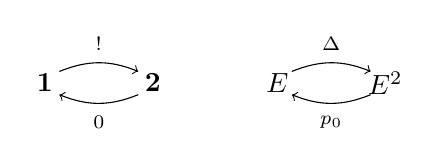
\begin{tikzpicture}[x=1.5em,y=1.5em]
  \node (o1) at (0,0) {$\qcOne$};
  \node (o2) at (2.6,0) {$\qcTwo$};
  \draw[->] (0.35,0.28) to[bend left=22] (2.25,0.28);
  \node at (1.3,0.95) {$\scriptstyle!$};
  \draw[->] (2.25,-0.28) to[bend left=22] (0.35,-0.28);
  \node at (1.3,-0.95) {$\scriptstyle 0$};
  \node at (4.3,0) {$\rightsquigarrow$};
  \begin{scope}[shift={(5.6,0)}]
  \node (E)  at (0,0) {$E$};
  \node (E2) at (2.6,0) {$E^{2}$};
  \draw[->] (0.35,0.28) to[bend left=22] (2.25,0.28);
  \node at (1.3,0.95) {$\scriptstyle\Delta$};
  \draw[->] (2.25,-0.28) to[bend left=22] (0.35,-0.28);
  \node at (1.3,-0.95) {$\scriptstyle p_{0}$};
  \end{scope}
\end{tikzpicture}
\end{center}
特别地，由第 2 章中的引理 2.3.7，\trCounit{} $\nu\colon\Delta p_{0}\Rightarrow\mathrm{id}$
定义了恒同沿 $\Delta$ 的一个绝对右提升。由第 2 章中的引理 2.4.1，这一绝对提升图
与 (ii) 的绝对提升图复合，定义出满足 (iii) 所要求性质的绝对提升图：
\begin{center}
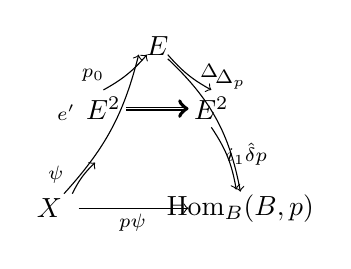
\begin{tikzpicture}[x=1.5em,y=1.5em]
  \node (E)   at (2.6,2.7) {$E$};
  \node (E2a) at (1.3,1.2) {$E^{2}$};
  \node (E2b) at (3.9,1.2) {$E^{2}$};
  \node (X)   at (0,-1.2) {$X$};
  \node (HB)  at (4.6,-1.2) {$\mathrm{Hom}_{B}(B,p)$};
  \draw[->] (0.35,-0.85) to[bend right=14] (2.15,2.5);
  \node at (0.4,1.1) {$\scriptstyle e'$};
  \draw[->] (1.3,1.65) to[bend right=10] (2.35,2.5);
  \node at (1.05,2.0) {$\scriptstyle p_{0}$};
  \draw[->] (2.85,2.5) to[bend right=10] (3.9,1.65);
  \node at (3.85,2.1) {$\scriptstyle\Delta$};
  \draw[double,->] (1.85,1.2) -- (3.35,1.2);
  \draw[->] (0.7,-1.2) -- (3.35,-1.2);
  \node at (2.0,-1.55) {$\scriptstyle\qcor{p\psi}$};
  \draw[->] (0.55,-0.85) to[bend left=10] (1.1,-0.1);
  \node at (0.15,-0.4) {$\scriptstyle\qcor{\psi}$};
  \draw[->] (3.9,0.75) to[bend left=12] (4.5,-0.75);
  \node at (4.75,0.1) {$\scriptstyle i_{1}\hat{\delta}p$};
  \draw[->] (2.85,2.4) to[bend left=18] (4.6,-0.8);
  \node at (4.35,1.9) {$\scriptstyle\Delta_{p}$};
\end{tikzpicture}
\end{center}

\textbf{(iii)$\Rightarrow$(i)：}由定理 3.5.3，一个绝对右提升图表——如 (iii)
所给出的——供应一个\trFiberedEquivalence。对如下左侧的泛型绝对右提升图表，
\trFiberedEquivalence{} $\mathrm{Hom}_{B}(B,r)\simeq_{C\times B}\mathrm{Hom}_{A}(f,g)$
可以通过复合如下右侧图中的诸虚映射来构造——也就是把该映射构造成点线复合映射的%
一个限制（见第 2 章中的引理 2.1.14）：
\begin{center}
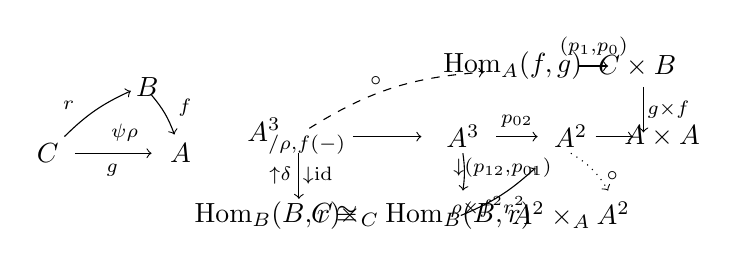
\begin{tikzpicture}[x=1.5em,y=1.5em]
  \node (B) at (2.4,1.6) {$B$};
  \node (C) at (0,0) {$C$};
  \node (A) at (3.2,0) {$A$};
  \draw[->] (0.4,0.4) to[bend left=10] (2.0,1.5);
  \node at (0.5,1.15) {$\scriptstyle r$};
  \draw[->] (2.5,1.4) to[bend left=10] (3.05,0.45);
  \node at (3.3,1.1) {$\scriptstyle f$};
  \draw[->] (0.65,0) -- (2.5,0);
  \node at (1.55,-0.4) {$\scriptstyle g$};
  \node at (1.85,0.5) {$\scriptstyle\psi\rho$};
  \node at (4.6,0.8) {$\rightsquigarrow$};
  \begin{scope}[shift={(5.6,0)}]
  \node (Hfg) at (5.6,2.1) {$\mathrm{Hom}_{A}(f,g)$};
  \node (CB)  at (8.6,2.1) {$C\times B$};
  \draw[->] (7.2,2.1) -- node[above]{$\scriptstyle(p_{1},p_{0})$} (7.9,2.1);
  \node at (7.5,1.75) {$\scriptstyle\llcorner$};
  \draw[->] (8.75,1.6) -- (8.75,0.5);
  \node at (9.35,1.05) {$\scriptstyle g\times f$};
  \draw[->,dashed] (0.7,0.6) to[bend left=14] (4.9,1.95);
  \node at (2.3,1.75) {$\scriptstyle\circ$};
  \node (A3) at (0.4,0.4) {$A^{3}_{/\rho,f(-)}$};
  \draw[->] (1.75,0.4) -- (3.4,0.4);
  \node (A3b) at (4.4,0.4) {$A^{3}$};
  \draw[->] (5.2,0.4) -- node[above]{$\scriptstyle p_{02}$} (6.2,0.4);
  \node (A2) at (7.0,0.4) {$A^{2}$};
  \draw[->] (7.6,0.4) -- (8.5,0.4);
  \node (AA) at (9.2,0.4) {$A\times A$};
  \draw[->] (0.45,0.0) -- (0.45,-1.1);
  \node at (0.0,-0.55) {$\scriptstyle\uparrow\delta$};
  \node at (0.9,-0.55) {$\scriptstyle\downarrow\mathrm{id}$};
  \draw[->] (4.4,0.0) to[bend left=8] (4.4,-0.9);
  \node at (5.35,-0.35) {$\scriptstyle\downarrow(p_{12},p_{01})$};
  \draw[->,dotted] (7.0,0.0) to[bend left=14] (7.9,-0.9);
  \node at (8.0,-0.55) {$\scriptstyle\circ$};
  \node (HB) at (-0.3,-1.5) {$\mathrm{Hom}_{B}(B,r)$};
  \node (iso) at (1.6,-1.5) {$\cong$};
  \node (CH) at (3.4,-1.5) {$C\times_{C}\mathrm{Hom}_{B}(B,r)$};
  \draw[->] (4.35,-1.5) to[bend right=10] (6.15,-0.35);
  \node at (5.0,-1.3) {$\scriptstyle\qcor{\rho}\times f^{2}r^{2}$};
  \node (A22) at (7.0,-1.5) {$A^{2}\times_{A}A^{2}$};
  \end{scope}
\end{tikzpicture}
\end{center}
由\trTwoOfThreeProperty，限制映射
$\circ\colon A^{3}_{/\rho,f(-)}\twoheadrightarrow\mathrm{Hom}_{A}(f,g)$
是一个\trEquivalence。

应用于 (iii) 的绝对右提升图表，这就构造出一条\trTrivialFibration
\begin{rveq}\label{eq:restriction-trivial-fibration}
\mathrm{Hom}_{B}(B,p)^{3}_{(\epsilon,\Delta_{p}(-))}
\xrightarrow[\ ]{\ p_{02}\ }
\mathrm{Hom}_{\mathrm{Hom}_{B}(B,p)}(\Delta_{p},\qcor{p\psi})
\end{rveq}
\eqref{eq:restriction-trivial-fibration} 的定义域是下图表演算出的极限——先拉回%
各行、再对所得\trCospan{}取\trPullback：
\begin{center}
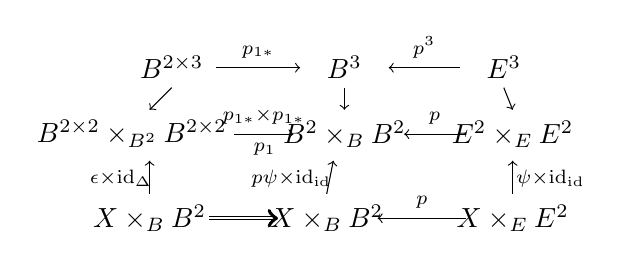
\begin{tikzpicture}[x=1.6em,y=1.6em]
  \node (b23) at (1.5,2.4) {$B^{2\times 3}$};
  \node (b3)  at (5.4,2.4) {$B^{3}$};
  \node (e3)  at (9.0,2.4) {$E^{3}$};
  \draw[->] (2.5,2.4) -- node[above]{$\scriptstyle p_{1*}$} (4.4,2.4);
  \draw[->] (8.0,2.4) -- node[above]{$\scriptstyle p^{3}$} (6.4,2.4);
  \node (b22) at (0.6,0.9) {$B^{2\times 2}\times_{B^{2}}B^{2\times 2}$};
  \node (b22b) at (5.4,0.9) {$B^{2}\times_{B}B^{2}$};
  \node (e22) at (9.2,0.9) {$E^{2}\times_{E}E^{2}$};
  \draw[->] (2.9,0.9) -- node[above]{$\scriptstyle p_{1*}\times p_{1*}$} (4.25,0.9);
  \node at (3.6,0.55) {$\scriptstyle p_{1}$};
  \draw[->] (8.15,0.9) -- node[above]{$\scriptstyle p^{\llcorner}$} (6.75,0.9);
  \node (xb) at (1.0,-1.0) {$X\times_{B}B^{2}$};
  \node (xb2) at (5.0,-1.0) {$X\times_{B}B^{2}$};
  \node (xe)  at (9.2,-1.0) {$X\times_{E}E^{2}$};
  \draw[double,->] (2.35,-1.0) -- (3.9,-1.0);
  \draw[->] (8.15,-1.0) -- node[above]{$\scriptstyle p$} (6.15,-1.0);
  \draw[->] (1.0,-0.45) -- (1.0,0.3);
  \node at (0.35,-0.1) {$\scriptstyle\qcor{\epsilon}\times\mathrm{id}_{\Delta}$};
  \draw[->] (5.0,-0.45) -- (5.15,0.3);
  \node at (4.2,-0.1) {$\scriptstyle\qcor{p\psi}\times\mathrm{id}_{\mathrm{id}}$};
  \draw[->] (9.2,-0.45) -- (9.2,0.3);
  \node at (10.05,-0.1) {$\scriptstyle\qcor{\psi}\times\mathrm{id}_{\mathrm{id}}$};
  \draw[->] (1.5,1.95) -- (1.0,1.45);
  \draw[->] (5.4,1.95) -- (5.4,1.45);
  \draw[->] (9.0,1.95) -- (9.2,1.45);
\end{tikzpicture}
\end{center}
但由超立方体拉回引理，它同样可以取成诸列的\trPullback{}之间诱导出的那个%
\trCospan{}的\trPullback：
\[
\mathrm{Hom}_{B}(B,pe')\times_{B^{2\times\llcorner}}B^{2\times 3}
\xrightarrow{\ p_{1*}\ }\ B_{/p\psi}
\xleftarrow{\ p\ }\ E_{/\psi}
\]
于是我们要寻求对左手列之\trPullback{}的更好理解。

由于 $\epsilon\colon\Delta_{p}e'\Rightarrow\qcor{p\psi}$满足%
$p_{0}\epsilon=\mathrm{id}_{pe'}$，我们可以选取一个表示\trFunctor{}
$\qcor{\epsilon}$，使其穿过如下\trPullback
\begin{center}
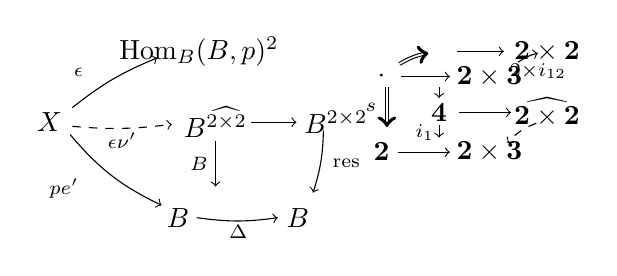
\begin{tikzpicture}[x=1.5em,y=1.5em]
  \node (HB2) at (3.6,2.5) {$\mathrm{Hom}_{B}(B,p)^{2}$};
  \node (X)   at (0,0.8) {$X$};
  \node (Bh)  at (4.0,0.8) {$B^{\widehat{2\times 2}}$};
  \node (B22) at (6.9,0.8) {$B^{2\times 2}$};
  \draw[->] (0.55,1.15) to[bend left=8] (2.6,2.35);
  \node at (0.7,2.0) {$\scriptstyle\qcor{\epsilon}$};
  \draw[->,dashed] (0.55,0.7) to[bend right=6] (2.95,0.75);
  \node at (1.75,0.35) {$\scriptstyle\qcor{\epsilon\nu'}$};
  \draw[->] (4.85,0.8) -- (5.95,0.8);
  \node at (5.35,1.1) {$\scriptstyle\llcorner$};
  \draw[->] (4.0,0.35) -- (4.0,-0.75);
  \node at (3.6,-0.2) {$\scriptstyle B$};
  \draw[->] (0.5,0.5) to[bend right=12] (2.7,-1.2);
  \node at (0.35,-0.8) {$\scriptstyle pe'$};
  \node (B) at (3.1,-1.5) {$B$};
  \draw[->] (3.55,-1.5) to[bend right=8] (5.5,-1.5);
  \node at (4.55,-1.85) {$\scriptstyle\Delta$};
  \node (Bg) at (6.0,-1.5) {$B^{\ulcorner}$};
  \draw[->] (6.6,0.6) to[bend left=8] (6.35,-0.9);
  \node at (7.15,-0.2) {$\scriptstyle\mathrm{res}$};
  \begin{scope}[shift={(8.0,0.6)},x=1.3em,y=1.3em]
  \node (G)  at (1.6,2.2) {$\ulcorner$};
  \node (T22) at (4.6,2.2) {$\qcTwo\times\qcTwo$};
  \draw[->] (2.1,2.2) -- (3.4,2.2);
  \node (qb) at (0,1.5) {$\boxdot\cdot$};
  \node (T23) at (3.0,1.5) {$\qcTwo\times\qcThree$};
  \draw[->,double] (0.5,1.85) to[bend left=10] (1.3,2.15);
  \draw[->] (0.55,1.5) -- (1.9,1.5);
  \draw[->] (3.8,1.9) to[bend left=10] (4.35,2.15);
  \node at (4.35,1.65) {$\scriptstyle 2\times i_{12}$};
  \node (T4) at (1.6,0.5) {$\qcFour$};
  \draw[->] (1.6,1.2) -- (1.6,0.9);
  \draw[->,double] (0.15,1.2) -- (0.15,0.1);
  \node at (-0.3,0.65) {$\scriptstyle s$};
  \node (t2) at (0,-0.6) {$\qcTwo$};
  \draw[->] (1.6,0.15) -- (1.6,-0.2);
  \node at (1.2,-0.05) {$\scriptstyle i_{1}$};
  \node (T2h) at (4.6,0.5) {$\widehat{\qcTwo\times\qcTwo}$};
  \draw[->] (2.15,0.5) -- (3.6,0.5);
  \node at (2.85,0.8) {$\scriptstyle\ulcorner$};
  \draw[->,dashed] (4.3,0.2) to[bend right=14] (3.5,-0.35);
  \node (T23b) at (3.0,-0.6) {$\qcTwo\times\qcThree$};
  \draw[->] (0.45,-0.6) -- (1.9,-0.6);
  \node at (1.15,-0.3) {$\scriptstyle\ulcorner$};
  \end{scope}
\end{tikzpicture}
\end{center}
——它由按立方体后面中单纯集的\trPushout{}所指示的方式，退化 $2\times 2$ 中的始%
\trCospan{}而得。沿 $\Delta\colon B^{2}\to B^{2\times 2}$拉回，则在 $2\times 3$
的左手方块中实现了一种类似的取商，如立方体的前面所示，其中 $s\colon\boxdot\cdot\to\qcTwo$
把左侧两个对象送到 $0$、把右侧三个对象送到 $1$。于是我们看到，映射%
\eqref{eq:restriction-trivial-fibration}定义为沿 $\qcor{\epsilon'}$对下图中的%
映射 $q$ 取\trPullback：
\begin{center}
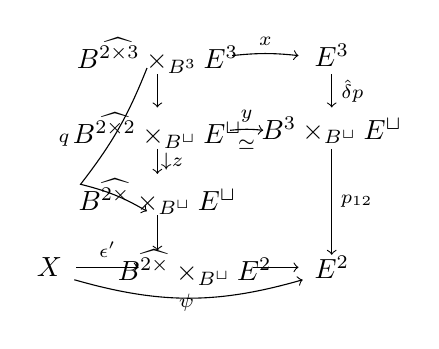
\begin{tikzpicture}[x=1.5em,y=1.5em]
  \node (t1) at (2.6,3.2) {$B^{\widehat{2\times 3}}\times_{B^{3}}E^{3}$};
  \node (E3) at (6.8,3.2) {$E^{3}$};
  \draw[->] (4.4,3.2) to[bend left=6] (6.0,3.2);
  \node at (5.2,3.55) {$\scriptstyle x$};
  \draw[->] (2.6,2.75) -- (2.6,1.95);
  \draw[->] (6.8,2.75) -- (6.8,1.95);
  \node at (7.3,2.35) {$\scriptstyle\hat{\delta}p$};
  \node (m1) at (2.6,1.4) {$B^{\widehat{2\times 2}}\times_{B^{\sqcup}}E^{\sqcup}$};
  \node (m2) at (6.8,1.4) {$B^{3}\times_{B^{\sqcup}}E^{\sqcup}$};
  \draw[->] (4.35,1.4) to[bend left=6] (5.15,1.4);
  \node at (4.75,1.75) {$\scriptstyle y$};
  \node at (4.75,1.05) {$\scriptstyle\simeq$};
  \draw[->] (2.6,0.95) -- (2.6,0.35);
  \node at (2.95,0.65) {$\scriptstyle\downarrow z$};
  \draw[->] (6.8,0.95) -- (6.8,-1.6);
  \node at (7.4,-0.3) {$\scriptstyle p_{12}$};
  \node (l3) at (2.6,-0.2) {$B^{\widehat{2\times\llcorner}}\times_{B^{\sqcup}}E^{\sqcup}$};
  \draw[->] (2.6,-0.65) -- (2.6,-1.5);
  \draw[->] (2.35,2.9) to[bend left=8] (0.75,0.1) to[bend left=8] (2.35,-0.55);
  \node at (0.35,1.15) {$\scriptstyle q$};
  \node (X)  at (0,-1.9) {$X$};
  \node (b2) at (3.5,-1.9) {$B^{\widehat{2\times\llcorner}}\times_{B^{\sqcup}}E^{2}$};
  \node (E2) at (6.8,-1.9) {$E^{2}$};
  \draw[->] (0.65,-1.9) -- node[above]{$\scriptstyle\qcor{\epsilon'}$} (2.15,-1.9);
  \draw[->] (4.9,-1.9) -- (6.0,-1.9);
  \draw[->] (0.6,-2.2) to[bend right=16] (6.1,-2.2);
  \node at (3.3,-2.75) {$\scriptstyle\qcor{\psi}$};
\end{tikzpicture}
\end{center}
我们宣称：被标记为 $x$、$y$ 与 $z$ 的那些映射都是\trTrivialFibration。于是，由%
等价的\trTwoOfThreeProperty{}可得：若 $q$ 沿 $\qcor{\epsilon'}$的\trPullback{}是一个%
\trEquivalence——如 (iii) 的绝对右提升图表所给出的——则 $\hat{\delta}p$ 沿%
$\qcor{\psi}$的\trPullback{}是一个\trEquivalence，这就证明了 (i)。

\trTrivialFibration{} $x$ 与 $y$ 都是限制映射%
$B^{\widehat{2\times 3}}\twoheadrightarrow B^{3}$的\trPullback，我们将证明后者%
是\trTrivialFibration。这是范畴 $\qcThree$、$\boxdot\cdot$、$2\times 3$ 之间的%
一列伴随，它们在商\trSimplicialSet{}之间
\begin{center}
\begin{tikzpicture}[x=1.1em,y=1.1em]
  \node at (0,0) {$\left\{\vcenter{\hbox{\begin{tikzpicture}[x=1.1em,y=1.1em]
    \node at (0,0) {$\scriptstyle 0$};
    \node at (1.6,0) {$\scriptstyle 1$};
    \node at (3.2,0) {$\scriptstyle 2$};
    \draw[->] (0.3,0) -- (1.2,0);
    \draw[->] (1.9,0) -- (2.8,0);
  \end{tikzpicture}}}\right\}$};
  \draw[->] (2.8,0.25) to[bend left=22] (5.4,0.25);
  \draw[->] (5.4,-0.25) to[bend left=22] (2.8,-0.25);
  \node at (4.1,0) {$\scriptstyle\perp$};
  \node at (6.9,0) {$\left\{\vcenter{\hbox{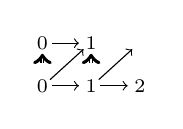
\begin{tikzpicture}[x=1.1em,y=1.1em]
    \node at (0,0.5) {$\scriptstyle 0$};
    \node at (1.6,0.5) {$\scriptstyle 1$};
    \node at (0,-0.9) {$\scriptstyle 0$};
    \node at (1.6,-0.9) {$\scriptstyle 1$};
    \node at (3.2,-0.9) {$\scriptstyle 2$};
    \draw[->] (0.3,0.5) -- (1.2,0.5);
    \draw[double,->] (0,-0.15) -- (0,0.15);
    \draw[double,->] (1.6,-0.15) -- (1.6,0.15);
    \draw[->] (0.3,-0.9) -- (1.2,-0.9);
    \draw[->] (1.9,-0.9) -- (2.8,-0.9);
    \draw[->] (0.25,-0.7) -- (1.35,0.3);
    \draw[->] (1.85,-0.7) -- (2.95,0.3);
  \end{tikzpicture}}}\right\}$};
  \draw[->] (11.6,0.25) to[bend left=22] (14.2,0.25);
  \draw[->] (14.2,-0.25) to[bend left=22] (11.6,-0.25);
  \node at (12.9,0) {$\scriptstyle\perp$};
  \node at (15.9,0) {$\left\{\vcenter{\hbox{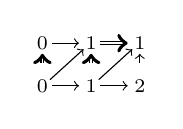
\begin{tikzpicture}[x=1.1em,y=1.1em]
    \node at (0,0.5) {$\scriptstyle 0$};
    \node at (1.6,0.5) {$\scriptstyle 1$};
    \node at (3.2,0.5) {$\scriptstyle 1$};
    \node at (0,-0.9) {$\scriptstyle 0$};
    \node at (1.6,-0.9) {$\scriptstyle 1$};
    \node at (3.2,-0.9) {$\scriptstyle 2$};
    \draw[->] (0.3,0.5) -- (1.2,0.5);
    \draw[double,->] (1.9,0.5) -- (2.8,0.5);
    \draw[double,->] (0,-0.15) -- (0,0.15);
    \draw[double,->] (1.6,-0.15) -- (1.6,0.15);
    \draw[->] (3.2,-0.15) -- (3.2,0.15);
    \draw[->] (0.3,-0.9) -- (1.2,-0.9);
    \draw[->] (1.9,-0.9) -- (2.8,-0.9);
    \draw[->] (0.25,-0.7) -- (1.35,0.3);
    \draw[->] (1.85,-0.7) -- (2.95,0.3);
  \end{tikzpicture}}}\right\}$};
\end{tikzpicture}
\end{center}
成为单纯\trHomotopyEquivalence。
于是，沿该复合包含的限制便定义出一个\trEquivalence{}
$B^{\widehat{2\times 3}}\twoheadrightarrow B^{3}$。映射 $z$ 是%
$B^{\widehat{2\times 3}}\twoheadrightarrow B^{\widehat{2\times\llcorner}}$的一个%
\trPullback，后者是\trTrivialFibration，因为包含%
$2\times\llcorner\hookrightarrow 2\times 3$可以由「特殊外号角」填充（见附录 D
中的定理 D.5.1 与推论 D.3.12）。
这样我们看到，\eqref{eq:restriction-trivial-fibration}与%
\cref{def:pcartesian-arrow}的映射等价，从而 $\psi$ 是 $p$-\trCartesian，
这就证明了 (iii)$\Rightarrow$(i)。
\end{proof}

注意，\eqref{eq:hypercube-weakly-cartesian} 的\trWeaklyCartesianSquare{}底下的%
那个\trCospan{}的数据由一个\trFunctor{} $\qcor{\beta}\colon X\to\mathrm{Hom}_{B}(B,p)$
确定，后者表示一个\trNaturalTransformation{} $\beta\colon b\Rightarrow pe$，
其余定义域沿一个指定的\trFunctor{} $e\colon X\to E$ 穿过 $p$。于是，追问这种%
形式的特定箭头是否具有余定义域为 $e$ 的 $p$-笛卡尔提升，就是切题的。

\begin{definition}[$p$-笛卡尔提升]\label{def:pcartesian-lifts}
设 $p\colon E\twoheadrightarrow B$ 为一条\trIsofibration。称箭头%
$\qcor{\psi}\colon X\to E^{2}$ \textbf{\trLifting}（lift）箭头%
$\qcor{\beta}\colon X\to\mathrm{Hom}_{B}(B,p)$，若左下的三角形交换：
\begin{center}
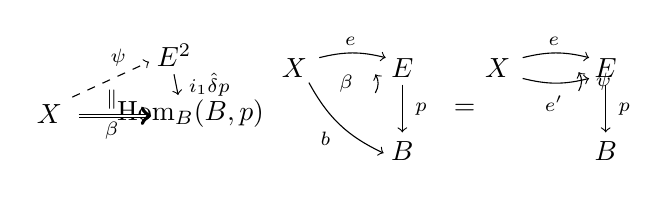
\begin{tikzpicture}[x=1.5em,y=1.5em]
  \node (E2) at (3.0,1.4) {$E^{2}$};
  \node (X)  at (0,0) {$X$};
  \node (HB) at (3.4,0) {$\mathrm{Hom}_{B}(B,p)$};
  \draw[->,dashed] (0.55,0.4) -- node[above,pos=0.6]{$\scriptstyle\qcor{\psi}$} (2.4,1.25);
  \draw[->] (3.0,0.95) -- (3.1,0.45);
  \node at (3.85,0.7) {$\scriptstyle i_{1}\hat{\delta}p$};
  \draw[double,->] (0.7,-0.05) -- (2.45,-0.05);
  \node at (1.5,-0.4) {$\scriptstyle\qcor{\beta}$};
  \node at (1.5,0.35) {$\scriptstyle\parallel$};
  \node at (4.9,0.7) {$\rightsquigarrow$};
  \begin{scope}[shift={(5.9,0)}]
  \node (X) at (0,1.1) {$X$};
  \node (E) at (2.6,1.1) {$E$};
  \node (B) at (2.6,-0.9) {$B$};
  \draw[->] (0.6,1.35) to[bend left=14] (2.2,1.35);
  \node at (1.35,1.75) {$\scriptstyle e$};
  \draw[->] (2.6,0.7) -- (2.6,-0.45);
  \node at (3.05,0.1) {$\scriptstyle p$};
  \draw[->] (0.35,0.75) to[bend right=18] (2.15,-0.95);
  \node at (0.75,-0.6) {$\scriptstyle b$};
  \draw[->] (1.95,0.5) to[bend right=30] (1.95,0.95);
  \node at (1.25,0.72) {$\scriptstyle\beta$};
  \node at (4.1,0.1) {$=$};
  \begin{scope}[shift={(4.9,0)}]
  \node (X) at (0,1.1) {$X$};
  \node (E) at (2.6,1.1) {$E$};
  \node (B) at (2.6,-0.9) {$B$};
  \draw[->] (0.6,1.35) to[bend left=14] (2.2,1.35);
  \node at (1.35,1.75) {$\scriptstyle e$};
  \draw[->] (0.6,0.85) to[bend right=14] (2.2,0.85);
  \node at (1.35,0.25) {$\scriptstyle e'$};
  \draw[->] (1.95,0.55) to[bend right=30] (1.95,1.0);
  \node at (2.55,0.78) {$\scriptstyle\psi$};
  \draw[->] (2.6,0.7) -- (2.6,-0.45);
  \node at (3.05,0.1) {$\scriptstyle p$};
  \end{scope}
  \end{scope}
\end{tikzpicture}
\end{center}
这给出\trHomotopyTwoCategory{}中的粘贴等式 $\beta=p\psi$。\footnote{提升性质
以\trHomotopyTwoCategory{}中的 2-胞腔来陈述，还是以∞-宇宙诸\trFunctorSpace{}%
中的 1-箭头来陈述，并无实质差别：见\cref{ex:homotopy-lifting}。}当%
$\qcor{\psi}$是 $p$-\trCartesian{}时，我们称它定义了 $\qcor{\beta}$ 的一个
\textbf{$p$-笛卡尔提升}（\emph{$p$-cartesian lift}）。
\end{definition}

$p$-笛卡尔变换的\trUniversalProperty{}蕴含：共同的\trNaturalTransformation{}
$\beta\colon b\Rightarrow pe$ 的任意两个 $p$-笛卡尔提升所表示的那些%
\trNaturalTransformation{}是\trFiberedIsomorphism{}的：

\begin{lemma}[笛卡尔提升的唯一性]\label{lem:uniqueness-of-cartesian-lifts}
若\trNaturalTransformation{}
\cellpair{X}{E}{e'}{e}{\psi}
与
\cellpair{X}{E}{e''}{e}{\psi'}
是共同的\trNaturalTransformation{} $\beta\colon b\Rightarrow pe$ 的%
$p$-笛卡尔提升，则存在一个可逆\trNaturalTransformation{}
\cellpair{X}{E}{e''}{e'}{\zeta}
使得 $\psi'=\psi\cdot\zeta$ 且 $p\zeta=\mathrm{id}_{b}$。
\end{lemma}

\begin{proof}
若 $\psi$ 与 $\psi'$ 定义出共同箭头 $\beta$ 的 $p$-笛卡尔提升，则由%
\cref{thm:pcartesian-characterizations}(iii) 我们有 $\qcor{\beta}$沿%
$\Delta_{p}$ 的一对绝对右提升 $(e',\epsilon)$ 与 $(e'',\epsilon')$，满足%
$p_{1}\epsilon=\psi$、$p_{1}\epsilon'=\psi'$，且%
$p_{0}\epsilon=\mathrm{id}_{b}=p_{0}\epsilon'$。由绝对右提升图表的单性，这诱导出%
一个自然同构
\begin{center}
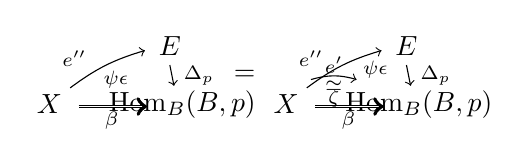
\begin{tikzpicture}[x=1.5em,y=1.5em]
  \node (E)  at (2.9,1.4) {$E$};
  \node (X)  at (0,0) {$X$};
  \node (HB) at (3.2,0) {$\mathrm{Hom}_{B}(B,p)$};
  \draw[->] (0.5,0.4) to[bend left=10] (2.3,1.3);
  \node at (0.6,1.1) {$\scriptstyle e''$};
  \draw[->] (2.9,0.95) -- (3.0,0.45);
  \node at (3.6,0.7) {$\scriptstyle\Delta_{p}$};
  \draw[double,->] (0.7,-0.05) -- (2.35,-0.05);
  \node at (1.5,-0.4) {$\scriptstyle\qcor{\beta}$};
  \node at (1.6,0.6) {$\scriptstyle\psi\epsilon$};
  \node at (4.7,0.7) {$=$};
  \begin{scope}[shift={(5.7,0)}]
  \node (E)  at (2.9,1.4) {$E$};
  \node (X)  at (0,0) {$X$};
  \node (HB) at (3.2,0) {$\mathrm{Hom}_{B}(B,p)$};
  \draw[->] (0.5,0.4) to[bend left=10] (2.3,1.3);
  \node at (0.6,1.1) {$\scriptstyle e''$};
  \draw[->] (2.9,0.95) -- (3.0,0.45);
  \node at (3.6,0.7) {$\scriptstyle\Delta_{p}$};
  \draw[double,->] (0.7,-0.05) -- (2.35,-0.05);
  \node at (1.5,-0.4) {$\scriptstyle\qcor{\beta}$};
  \draw[->] (0.6,0.6) to[bend left=16] (1.7,0.6);
  \node at (1.15,0.95) {$\scriptstyle e'$};
  \node at (1.15,0.15) {$\scriptstyle\zeta$};
  \node at (1.15,0.45) {$\scriptstyle\simeq$};
  \node at (2.15,0.85) {$\scriptstyle\psi\epsilon$};
  \end{scope}
\end{tikzpicture}
\end{center}
使得 $\epsilon'=\epsilon\cdot\Delta_{p}\zeta$。将此等式与 $p_{1}$ 作%
\trWhiskering{}可见 $\psi'=\psi\cdot\zeta$，而与 $p_{0}$ 作\trWhiskering{}可见%
$\mathrm{id}_{b}=p\zeta$。
\end{proof}

把这些结果结合起来，我们得到一个有用的保守性性质：

\begin{lemma}[笛卡尔保守性]\label{lem:cartesian-conservativity}
设有
\cellpair{X}{E}{e'}{e}{\psi}、
\cellpair{X}{E}{e''}{e}{\psi'}
与
\cellpair{X}{E}{e''}{e'}{\zeta}，
它们是\trNaturalTransformation，满足 $\psi$ 与 $\psi'$ 是 $p$-\trCartesian、%
$\psi'=\psi\cdot\zeta$，且 $p\zeta$ 可逆。则 $\zeta$ 可逆。
\end{lemma}

\begin{proof}
由\cref{lem:left-cancellation}与\cref{lem:isomorphism-stability}，$\zeta$ 是某个%
自然同构的 $p$-笛卡尔提升，因而必定可逆。
\end{proof}

刻画 $p$-笛卡尔变换的\cref{thm:pcartesian-characterizations}之\trUniversalProperty{}%
在同伦 2-范畴的层面上产生了归纳与保守性运算，与第 3 章中考虑过的那些运算类似。

\begin{proposition}[$p$-笛卡尔箭头的弱泛性质]\label{prop:pcartesian-weak-universal-property}
设 $p\colon E\twoheadrightarrow B$为\trIsofibration。一支 $p$-笛卡尔箭头
\cellpair{X}{E}{e'}{e}{\psi}
在\trHomotopyTwoCategory{}中具有由以下两种运算给出的弱\trUniversalProperty：
\begin{enumerate}[label=(\roman*)]
\item \textbf{归纳：}给定任意 2-胞腔
\cellpair{X}{E}{e''}{e}{\tau}
与
\cellpair{X}{B}{pe''}{pe'}{\gamma}，
使得 $p\tau=p\psi\cdot\gamma$，则存在 $\gamma$ 的一个\trLifting{}
\cellpair{X}{E}{e''}{e'}{\bar{\gamma}}
使得 $\tau=\psi\cdot\bar{\gamma}$：
\begin{center}
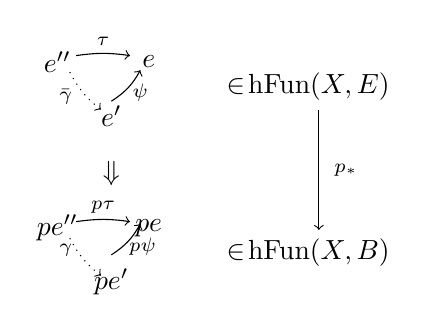
\begin{tikzpicture}[x=1.5em,y=1.5em]
  \node (e2) at (0,1.3) {$e''$};
  \node (e)  at (2.2,1.3) {$e$};
  \draw[->] (0.45,1.45) to[bend left=8] (1.75,1.45);
  \node at (1.1,1.8) {$\scriptstyle\tau$};
  \draw[->,dotted] (0.3,1.05) to[bend right=12] (1.05,0.15);
  \node at (0.2,0.45) {$\scriptstyle\bar{\gamma}$};
  \draw[->] (1.3,0.35) to[bend right=14] (2.0,1.1);
  \node at (2.0,0.55) {$\scriptstyle\psi$};
  \node (ep) at (1.3,0.0) {$e'$};
  \node at (4.3,0.7) {$\in$};
  \node at (6.3,0.7) {$\mathrm{hFun}(X,E)$};
  \node at (1.3,-1.4) {$\Downarrow$};
  \node (pe2) at (0,-2.7) {$pe''$};
  \node (pe)  at (2.2,-2.7) {$pe$};
  \draw[->] (0.45,-2.55) to[bend left=8] (1.75,-2.55);
  \node at (1.1,-2.2) {$\scriptstyle p\tau$};
  \draw[->,dotted] (0.3,-2.95) to[bend right=12] (1.05,-3.85);
  \node at (0.2,-3.25) {$\scriptstyle\gamma$};
  \draw[->] (1.3,-3.35) to[bend right=14] (2.0,-2.6);
  \node at (2.05,-3.15) {$\scriptstyle p\psi$};
  \node (pep) at (1.3,-4.0) {$pe'$};
  \node at (4.3,-3.3) {$\in$};
  \node at (6.3,-3.3) {$\mathrm{hFun}(X,B)$};
  \draw[->] (6.3,0.15) -- (6.3,-2.75);
  \node at (6.95,-1.3) {$\scriptstyle p_{*}$};
\end{tikzpicture}
\end{center}
\item \textbf{保守性：}$\psi$ 的任何纤维化自同态皆可逆：若%
$\zeta\colon e'\Rightarrow e'$是任一满足 $\psi\cdot\zeta=\psi$ 且%
$p\zeta=\mathrm{id}_{pe'}$的\trNaturalTransformation，则 $\zeta$ 可逆。
\end{enumerate}
\end{proposition}

\begin{proof}
保守性性质 (ii) 是\cref{lem:cartesian-conservativity}中观察到的保守性结果的
一个特例，故只需证 (i)。

偶对 $\tau\colon e''\Rightarrow e$ 与 $\gamma\colon pe''\Rightarrow pe'$
满足第 3 章中的命题 3.4.6 所要求的相容性条件，从而诱导出如下左侧的%
\trNaturalTransformation{} $\sigma$，满足 $p_{1}\sigma=\tau$ 与%
$p_{0}\sigma=\gamma$。由于 $\psi$ 是 $p$-\trCartesian，此 2-胞腔穿过%
\cref{thm:pcartesian-characterizations}(iii) 的绝对右提升图表分解：
\begin{center}
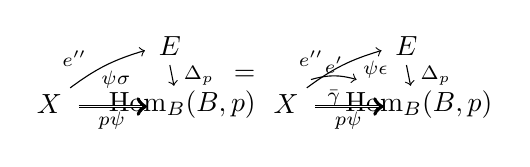
\begin{tikzpicture}[x=1.5em,y=1.5em]
  \node (E)  at (2.9,1.4) {$E$};
  \node (X)  at (0,0) {$X$};
  \node (HB) at (3.2,0) {$\mathrm{Hom}_{B}(B,p)$};
  \draw[->] (0.5,0.4) to[bend left=10] (2.3,1.3);
  \node at (0.6,1.1) {$\scriptstyle e''$};
  \draw[->] (2.9,0.95) -- (3.0,0.45);
  \node at (3.6,0.7) {$\scriptstyle\Delta_{p}$};
  \draw[double,->] (0.7,-0.05) -- (2.35,-0.05);
  \node at (1.5,-0.4) {$\scriptstyle\qcor{p\psi}$};
  \node at (1.6,0.6) {$\scriptstyle\psi\sigma$};
  \node at (4.7,0.7) {$=$};
  \begin{scope}[shift={(5.7,0)}]
  \node (E)  at (2.9,1.4) {$E$};
  \node (X)  at (0,0) {$X$};
  \node (HB) at (3.2,0) {$\mathrm{Hom}_{B}(B,p)$};
  \draw[->] (0.5,0.4) to[bend left=10] (2.3,1.3);
  \node at (0.6,1.1) {$\scriptstyle e''$};
  \draw[->] (2.9,0.95) -- (3.0,0.45);
  \node at (3.6,0.7) {$\scriptstyle\Delta_{p}$};
  \draw[double,->] (0.7,-0.05) -- (2.35,-0.05);
  \node at (1.5,-0.4) {$\scriptstyle\qcor{p\psi}$};
  \draw[->] (0.6,0.6) to[bend left=16] (1.7,0.6);
  \node at (1.15,0.95) {$\scriptstyle e'$};
  \node at (1.15,0.15) {$\scriptstyle\bar{\gamma}$};
  \node at (2.15,0.85) {$\scriptstyle\psi\epsilon$};
  \end{scope}
\end{tikzpicture}
\end{center}
由于 $(e',\epsilon)$ 是绝对右提升，$(e'',\sigma)$ 诱导出一个%
\trNaturalTransformation{} $\bar{\gamma}\colon e''\Rightarrow e'$，使得%
$\sigma=\epsilon\cdot\Delta_{p}\bar{\gamma}$。将这些等式与 $p_{1}$ 作%
\trWhiskering{}可见 $\tau=\psi\cdot\bar{\gamma}$，而与 $p_{0}$ 作%
\trWhiskering{}可见 $\gamma=p\bar{\gamma}$。
\end{proof}

\cref{prop:pcartesian-weak-universal-property}所列举的诸\trUniversalProperty{}%
远弱于\cref{def:pcartesian-arrow}所表达的那一个。的确，它们既不表达%
\cref{lem:cartesian-conservativity}中观察到的完整保守性，也没有利用笛卡尔变换与
绝对右提升图表的限制稳定性。尽管如此，在 $p$ 是\trCartesianFibration{}的条件下，
条件 (i) 与 (ii) 已足以刻画 $p$-笛卡尔变换类——\trCartesianFibration{}这一概念
将在下一节引入。更出人意料的是，若以一条限制稳定性性质增强 (i) 与 (ii)，命题
5.2.11 表明，完全可以仅从\trHomotopyTwoCategory{}的视角定义%
\trCartesianFibration，而无需援引\cref{def:pcartesian-arrow}。然而，即便在%
$p$ 本身并非\trCartesianFibration{}的情形下（例如见%
\cref{ex:codomain-projection-cartesian-arrows}），$p$-笛卡尔箭头也自有其独立的
研究价值；此时我们把笛卡尔纤维化理论的纯 2-范畴式发展置于次要地位，转而请读者
查阅 [110]。


\subsection*{练习}

\begin{exercise}\label{ex:homotopy-lifting}
回忆：\trInfinityCosmos{}中的诸箭头 $\qcor{\psi}\colon X\to E^{2}$对应于\trFunctorSpace{}
$\mathrm{Fun}(X,E)$ 中的一些 1-\trSimplex{}（亦即 1-箭头）$\psi\colon e'\to e$，
而一平行 1-箭头对表示同一个 2-胞腔
\cellpair{X}{E}{e'}{e}{\psi}
当且仅当二者\trHomotopic——即在 $\mathrm{Fun}(X,E)$ 中围出一条 2-箭头，
其第 0 条或第 2 条棱是退化的（见练习 3.2.i）。
证明：若 $p\colon E\twoheadrightarrow B$是一条\trIsofibration，使得每个%
\trNaturalTransformation{} $\beta\colon b\Rightarrow pe$ 在%
\trHomotopyTwoCategory{}中都容有一个\trLifting{} $\psi\colon e'\Rightarrow e$，
则 $\mathrm{Fun}(X,B)$ 中的每支 1-箭头 $\qcor{\beta}\colon b\to pe$ 都按%
\cref{def:pcartesian-lifts}的意义容有一个 1-箭头\trLifting{} $\psi\colon e'\to e$。
\end{exercise}

\begin{exercise}\label{ex:codomain-projection-cartesian-arrows}
（5.2.10）
\begin{enumerate}[label=(\roman*)]
\item 刻画余定义域投影函子 $p_{1}\colon A^{2}\twoheadrightarrow A$的%
\trCartesianArrow。
\item 用 (i) 的答案给出第 4 章中的命题 4.3.11 的另一个证明。
\end{enumerate}
\end{exercise}
